\documentclass{beamer}
% \documentclass[notes]{beamer}

\usetheme[progressbar=foot, block=fill]{metropolis}

\usepackage{graphicx}
% \usepackage{booktabs}
% \usepackage{algorithm}
% \usepackage{algpseudocode}
\usepackage{subcaption}
\usepackage{caption}
\usepackage{pgf-pie}
% \usepackage{tikz}
% \usepackage{upgreek}
\usepackage{appendixnumberbeamer}
\usepackage{subcaption}
\usepackage{cleveref}
\usepackage{amsmath}
\usepackage{amsfonts}
\usepackage{pgfplots}
% \usepackage{url}
\usepackage{xfrac}
\usepackage{appendixnumberbeamer}

% \usetikzlibrary{calc}
% \usetikzlibrary{3d}
\usetikzlibrary{spy,arrows}

% \usepackage{biblatex}
\usepackage[backend=biber,style=authoryear,natbib=true]{biblatex} % Use the bibtex backend with the authoryear citation style (which resembles APA)
\addbibresource{references.bib}

\graphicspath{ {images/} }

\title{Corner Localization and Camera Calibration from Imaged Lattices}
% \subtitle{A Novel Approach to Camera Calibration}
\author{Andrii Stadnik \inst{1} \and James Pritts \inst{2}}
\institute{
  \inst{1} Faculty of Computer Science, Ukrainian Catholic University, Lviv,
  Ukraine \\
  \inst{2} Czech Institute of Informatics, Robotics and Cybernetics at Czech Technical University in Prague, Czech
}
\date{2023}

% \metroset{}

\begin{document}

\begin{frame}
	\titlegraphic{\hfill
\includegraphics[height=1cm]{UCU-Apps2022_.png}}
	\titlepage
\end{frame}

\begin{frame}
	\frametitle{Structure of the presentation}
	\tableofcontents
\end{frame}

\section{Introduction}\label{sec:introduction}

\begin{frame}
	\frametitle{Camera calibration}

	Camera calibration is a necessary step for mapping from the pixel position to
	the real-world 3D position.

	\begin{alertblock}{Note}
		Here, we will use the term \textit{camera calibration} to refer to the
		geometric camera calibration.
	\end{alertblock}

	\begin{figure}
		\centering
		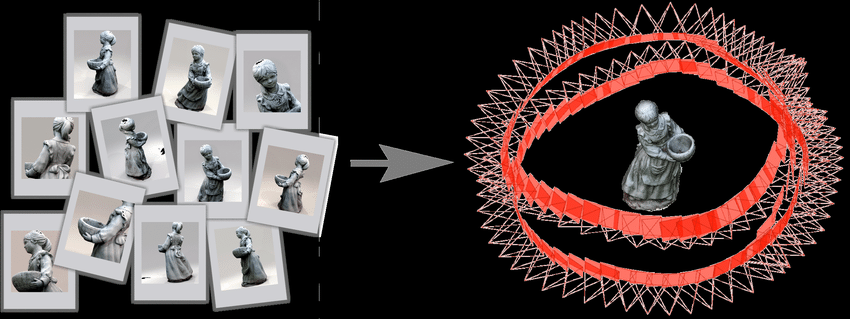
\includegraphics[width=0.8\textwidth]{3d_reconstruction.png}
		\caption{3D reconstruction}
	\end{figure}
\end{frame}

\begin{frame}
	\frametitle{Motivation}
	Accurate camera calibration is required for many applications, such as:
	\begin{itemize}
		\item 3D reconstruction
		\item Robotics and automation
		\item Augmented reality
		\item Photogrammetry
		\item Stereo vision
		\item And many more\ldots
	\end{itemize}
\end{frame}

\begin{frame}
	\frametitle{Challenges}
	% \begin{columns}[T,onlytextwidth]
	% \column{0.6\textwidth}
	Camera calibration is
	a challenging task, especially for highly distorted images.

	The challenges include:
	\begin{itemize}
		\item Robust keypoint detection
		\item Accurate distortion modeling
		\item Stability of the calibration
	\end{itemize}
\end{frame}

\begin{frame}
	\frametitle{Example}
	% \column{0.4\textwidth}
	\begin{figure}
		\begin{tikzpicture}[spy using outlines={circle,yellow,magnification=4,size=3cm, connect spies}]
			\node[anchor=south west,inner sep=0] (image) at (0,0)
			% {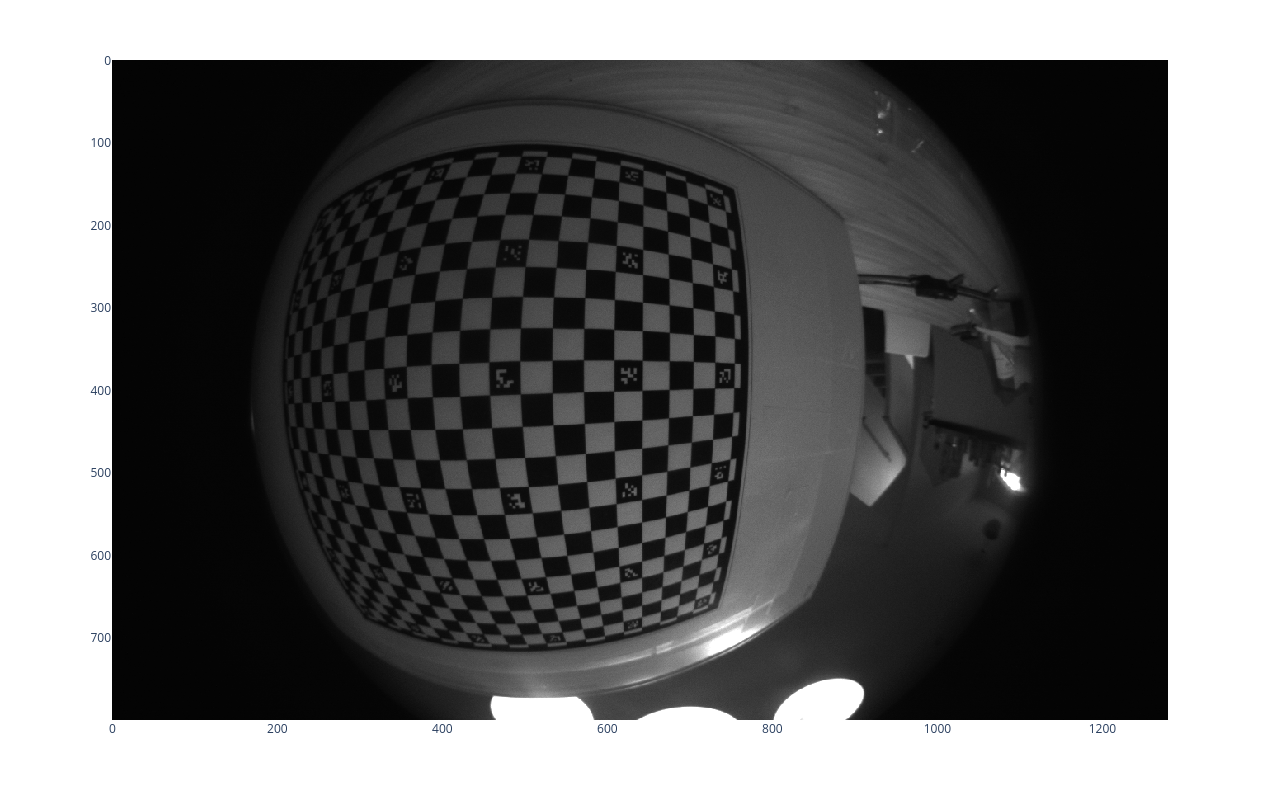
\includegraphics[width=0.6\textwidth]{distorted_image}};
			{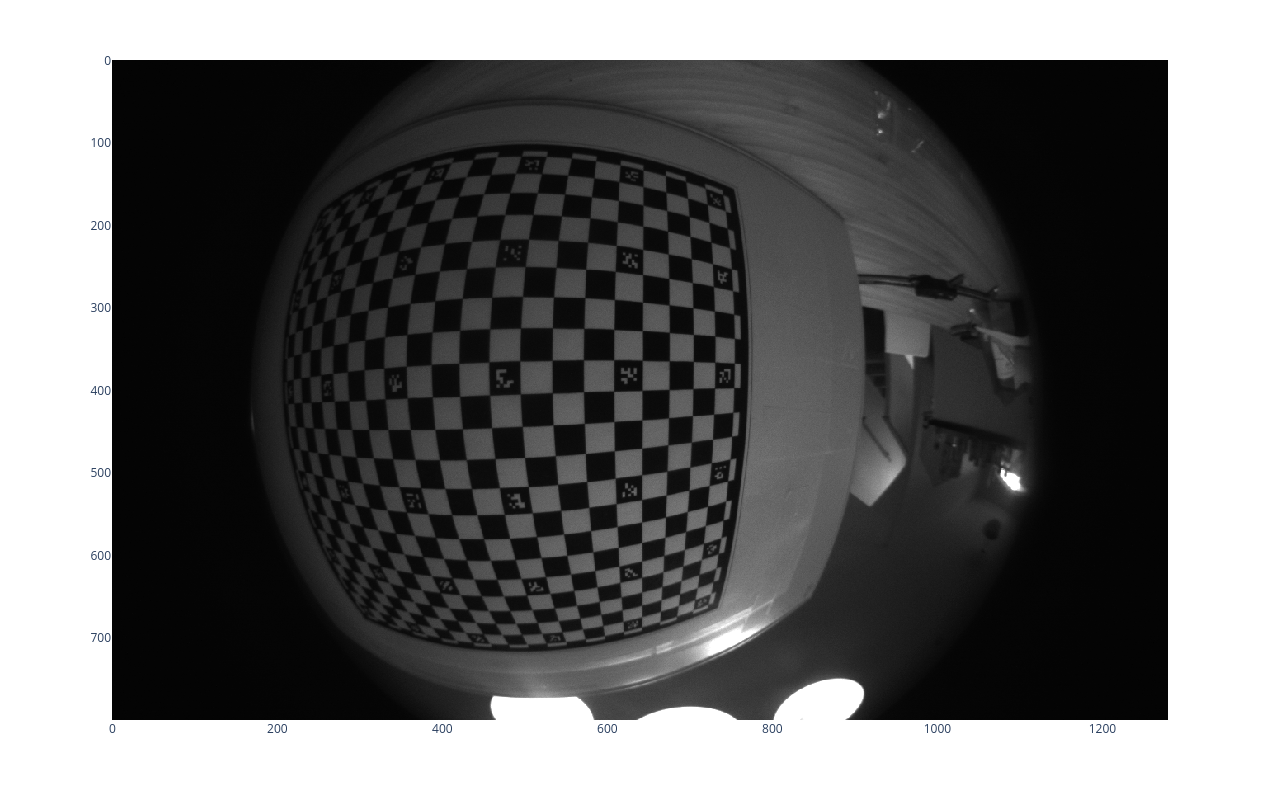
\includegraphics[width=0.8\textwidth]{distorted_image}};
			\begin{scope}[x={(image.south east)},y={(image.north west)}]
				\spy[red] on (2.5,1.4) in node [left] at (10.1,1.7);
				\spy[blue] on (3.5,3.0) in node [right] at (8.1,4.3);
			\end{scope}
		\end{tikzpicture}
		\caption{Example of corners near the center of the image and at the edge}
	\end{figure}
	% \end{columns}
\end{frame}

\begin{frame}
	\frametitle{Research objective}

	Improve the detection of
	calibration board fiducials from calibration imagery taken by wide-angle or
	fisheye lenses.

	% Add additional constrains to the camera
	% calibration by finding previously undetected features on the calibration
	% board.

	For that, we formulate the set of research questions:
	\begin{itemize}
		\item How to find additional features on the calibration board which were not
		      detected by the feature detector?
		\item How to filter out falsely detected features?
		\item Is there a need for finding additional features on the calibration
		      board? Are all of the points detected?
	\end{itemize}
\end{frame}

\section{Background}\label{sec:background}

\begin{frame}
	\frametitle{Notation}
	The column vectors will be denoted by bold lowercase letters (e.g.
	\(\mathbf{u} = \begin{pmatrix}
		u, v, 1
	\end{pmatrix}^{T}\)), matrices will be denoted by bold uppercase letters (e.g.
	\(H = \begin{bmatrix}
		\mathbf{r_1} & \mathbf{r_2} & \mathbf{t}
	\end{bmatrix}
	\)). We will use homogeneous coordinates to simplify the equations.
\end{frame}

\begin{frame}
	\frametitle{Camera model}
	Camera parameters can be divided into 3 parts:
	\begin{itemize}
		\item Extrinsic parameters
		\item Distortion parameters
		\item Intrinsic parameters
	\end{itemize}

	They define a camera model, which
	projects a homogeneous 3D scene point
	\(\mathbf{x} = \begin{pmatrix}
		x, y, z, 1
	\end{pmatrix}^{T}\) into the homogeneous image point
	\(\mathbf{u} = \begin{pmatrix}
		u, v, 1
	\end{pmatrix}^{T}\).
\end{frame}

\begin{frame}
	\frametitle{Definition of the camera model}
	\begin{exampleblock}{Definition}
		\begin{align}
			\alpha \mathbf{u} & = K f_{\boldsymbol{\lambda}}(H\mathbf{X})
			\tag{Projection} \label{eq:projection}                                            \\
			\alpha \mathbf{X} & = H^{-1} g_{\boldsymbol{\lambda}}(K^{-1}\mathbf{u}) \tag{Back
				projection} \label{eq:back_projection}.
		\end{align}
		where \(K\) is the camera matrix, \(g_{\boldsymbol{\lambda}}(\cdot)\) is the division distortion
		model \citep{fitzgibbonSimultaneousLinearEstimation2001}, \(f(\cdot)\) is the
		inverse of \(g(\cdot)\) and \(H\) is the homography matrix, and \(\alpha\)
		is a non-zero scalar.
	\end{exampleblock}

	\begin{alertblock}{Note}
		Slides with the detailed explanation can be demonstrated upon request during the Q\&A session.
		% The explanation of the used camera model does not fit into the
		% presentation duration. However, the appendix of this presentation contains
		% the detailed explanation of each element of the equation, and will be
		% happily discussed/presented during the Q\&A session.
	\end{alertblock}

\end{frame}

\section{Approach}\label{sec:approach}

\begin{frame}
	\frametitle{Pipeline overview}

	\begin{enumerate}
		\item Feature detection.
		\item Camera calibration.
		      \begin{enumerate}
			      \item Initialize camera parameters (\(R\), \(\mathbf{t}\),
			            \(\boldsymbol{\lambda}\)) using the solver.
			      \item Refine camera parameters and estimate \(K\) by optimization.
		      \end{enumerate}
		\item Impute the gaps in the board, and extend it.
		\item Get positions of new points on the image.
		\item Filter out false positives.
	\end{enumerate}
\end{frame}

\begin{frame}
	\frametitle{Feature detection}
	Use the approach, proposed by~\cite{geigerAutomaticCameraRange2012}:
	\begin{enumerate}
		\item Compute the corner likelihood map by convolving the image with two
		      \(n\times n\) prototypes.
		\item Additional filtering based on the number of the zero-crossings and
		      non-maximum suppression.
		\item Subpixel refinement of the detected corners.
		\item Board's structure refinement.
	\end{enumerate}
	\begin{figure}[h]
		\centering
		\begin{subfigure}{0.3\linewidth}
			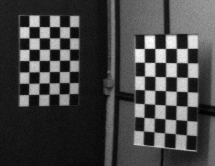
\includegraphics[width=\textwidth]{10.png}
			\caption{Input image}
		\end{subfigure}
		\begin{subfigure}{0.3\linewidth}
			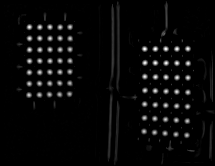
\includegraphics[width=\textwidth]{11.png}
			\caption{Corner likelihood}
		\end{subfigure}

		% \caption{Corner prototypes \citep{geigerAutomaticCameraRange2012}}
		\label{fig:corner_prototypes}
	\end{figure}

\end{frame}

\begin{frame}
	\frametitle{Camera calibration 1}

	\begin{enumerate}
		\item Initialize camera parameters (\(R\), \(\mathbf{t}\),
		      \(\boldsymbol{\lambda}\)) using the method, proposed by
		      \cite{scaramuzzaToolboxEasilyCalibrating2006}.
	\end{enumerate}
	\begin{exampleblock}{Overview}
		The author proposes the multistage solver for the projection equation,
		assuming that the camera matrix is known.
	\end{exampleblock}
\end{frame}

\begin{frame}
	\frametitle{Camera calibration 2}
	\begin{enumerate}
		\item Refine the values of \(R\), \(\mathbf{t}\), \(\boldsymbol{\lambda}\), and
		      estimate \(K\) by minimizing the reprojection error between the
		      board and the back-projected corners.
	\end{enumerate}

	\begin{exampleblock}{Reprojection error}
		The reprojection error is the distance between the reprojected point and the
		measured one:
		\begin{equation*}
			L = \sum_{i=1}^{N} \left\lVert
			H^{-1} g_{ \boldsymbol{\lambda}}(K^{-1} \mathbf{u_i}) -
			\mathbf{x_i} \right\rVert^2,
		\end{equation*}
		where \(\boldsymbol{\lambda}\) are the division distortion model
		parameters, \( \mathbf{x_{i}}\) and \(\mathbf{u_{i}}\) are the coordinates
		of the \(i\)-th corner in the 3D scene coordinates, and the respective
		feature on the image.
	\end{exampleblock}
\end{frame}

\begin{frame}
	\frametitle{Additional features detection}
	To find the probable positions of the previously undetected corners, we
	impute the gaps in the board, and extend it by 1 row and column from each
	side:
	\begin{figure}
		\begin{subfigure}{0.45\linewidth}
			\resizebox{\linewidth}{!}{
				\centering
				\begin{tikzpicture}
					\begin{axis}[
							xlabel={$x$},
							ylabel={$y$},
							grid=major,
							title={Original board},
						]
						\addplot[
							only marks,
						] table {data/original_board.txt};
					\end{axis}
				\end{tikzpicture}
			}
		\end{subfigure}
		\begin{subfigure}{0.45\linewidth}
			\resizebox{\linewidth}{!}{
				\centering
				\begin{tikzpicture}
					\begin{axis}[
							xlabel={$x$},
							ylabel={$y$},
							grid=major,
							title={Extended board},
						]
						\addplot[
							only marks,
						] table {data/extended_board.txt};
					\end{axis}
				\end{tikzpicture}
			}
		\end{subfigure}
	\end{figure}
\end{frame}

\begin{frame}
	\frametitle{Binary classification}
	\begin{itemize}
		\item Compute the corner likelihood map for the image.
		\item Use the ROC curve, and pick the threshold which maximizes the G-mean.
	\end{itemize}

	We tested the approach of \cite{geigerAutomaticCameraRange2012}, and,
	alternatively, the Hessian responses for the image, as proposed by
	\cite{chenNewSubPixelDetector2005}.
\end{frame}

\section{Experiments}\label{sec:experiments}

\begin{frame}
	\frametitle{Metrics}
	The paper's main contribution is finding additional calibration boards' features, which
	then can be used as an input to any other camera calibration algorithm.

	\begin{itemize}
		\item Number of recovered artificially removed points
		\item Number of recovered points under occlusion
		\item Number of recovered points on original images
	\end{itemize}

\end{frame}

\begin{frame}
	\frametitle{Dataset}
	\textbf{OV} \citep{lochmanBabelCalibUniversalApproach2021} is a dataset of
	approximately 1400 images. It was collected using eight stereo cameras.
	As a calibration pattern, the checkerboard pattern with \(9\times 6\) tags of 22 mm size
	was used.

	\begin{alertblock}{Note}
		Much more data was collected. However, the initial feature detection
		supports only checkerboard patterns for now. Other than that, the pipeline
		works with any pattern.
	\end{alertblock}
\end{frame}

\begin{frame}
	\frametitle{Camera calibration 1}
	Compare the initial camera calibration with camera calibration obtained via
	optimization of reprojection error.

	\begin{figure}
		\begin{subfigure}{0.45\linewidth}
			\resizebox{\linewidth}{!}{
				\begin{tikzpicture}
					\pie[rotate=90, explode=0.1, sum=auto, color={green!60, blue!60, red!60}, text=legend]{
						254/Correctly detected,
						80/Reprojection error > 10,
						458/Not correctly detected
					}
				\end{tikzpicture}
			}
			\caption{Initial calibration}
		\end{subfigure}
		\hfill
		\begin{subfigure}{0.45\linewidth}
			\resizebox{\linewidth}{!}{
				\begin{tikzpicture}
					\pie[rotate=90, explode=0.1, sum=auto, color={green!60, blue!60, red!60}, text=legend]{
						658/Correctly detected,
						19/Reprojection error > 10,
						115/Not correctly detected
					}
				\end{tikzpicture}
			}
			\caption{Final calibration}
		\end{subfigure}
	\end{figure}
\end{frame}

\begin{frame}
	\frametitle{Camera calibration 2}

	\begin{figure}
		% \begin{subfigure}{0.45\linewidth}
		\begin{subfigure}{\linewidth}
			\resizebox{\linewidth}{!}{
				\begin{tikzpicture}
					\begin{axis}[
							ybar interval,
							ymin=0,
							ylabel={Frequency},
							xlabel={Value},
							height=0.3\linewidth,
							width=\linewidth,
							ticklabel style = {font=\tiny},
							% title={Initial calibration}
						]
						\addplot+ [hist={data min=0,data max=10,bins=20}] table [y index=0]
							% \addplot+ [hist={bins=30}] table [y index=0]
							{data/reprojection_error_init.txt};
					\end{axis}
				\end{tikzpicture}
			}
			\caption{Initial calibration's reprojection error histogram}
		\end{subfigure}
		\begin{subfigure}{\linewidth}
			\resizebox{\linewidth}{!}{
				\begin{tikzpicture}
					\begin{axis}[
							ybar interval,
							ymin=0,
							ylabel={Frequency},
							xlabel={Value},
							height=0.3\linewidth,
							width=\linewidth,
							ticklabel style = {font=\tiny},
							% title={Reprojection error}
						]
						\addplot+ [hist={data min=0,data max=10,bins=20}] table [y index=0]
							% \addplot+ [hist={bins=30}] table [y index=0]
							{data/reprojection_error_final.txt};
					\end{axis}
				\end{tikzpicture}
			}
			\caption{Final calibration's reprojection error histogram (in px.)}
		\end{subfigure}
	\end{figure}

\end{frame}

\begin{frame}
	\frametitle{Additional features detection}

	\begin{columns}
		\begin{column}{0.6\textwidth}
			\begin{figure}
				\centering
				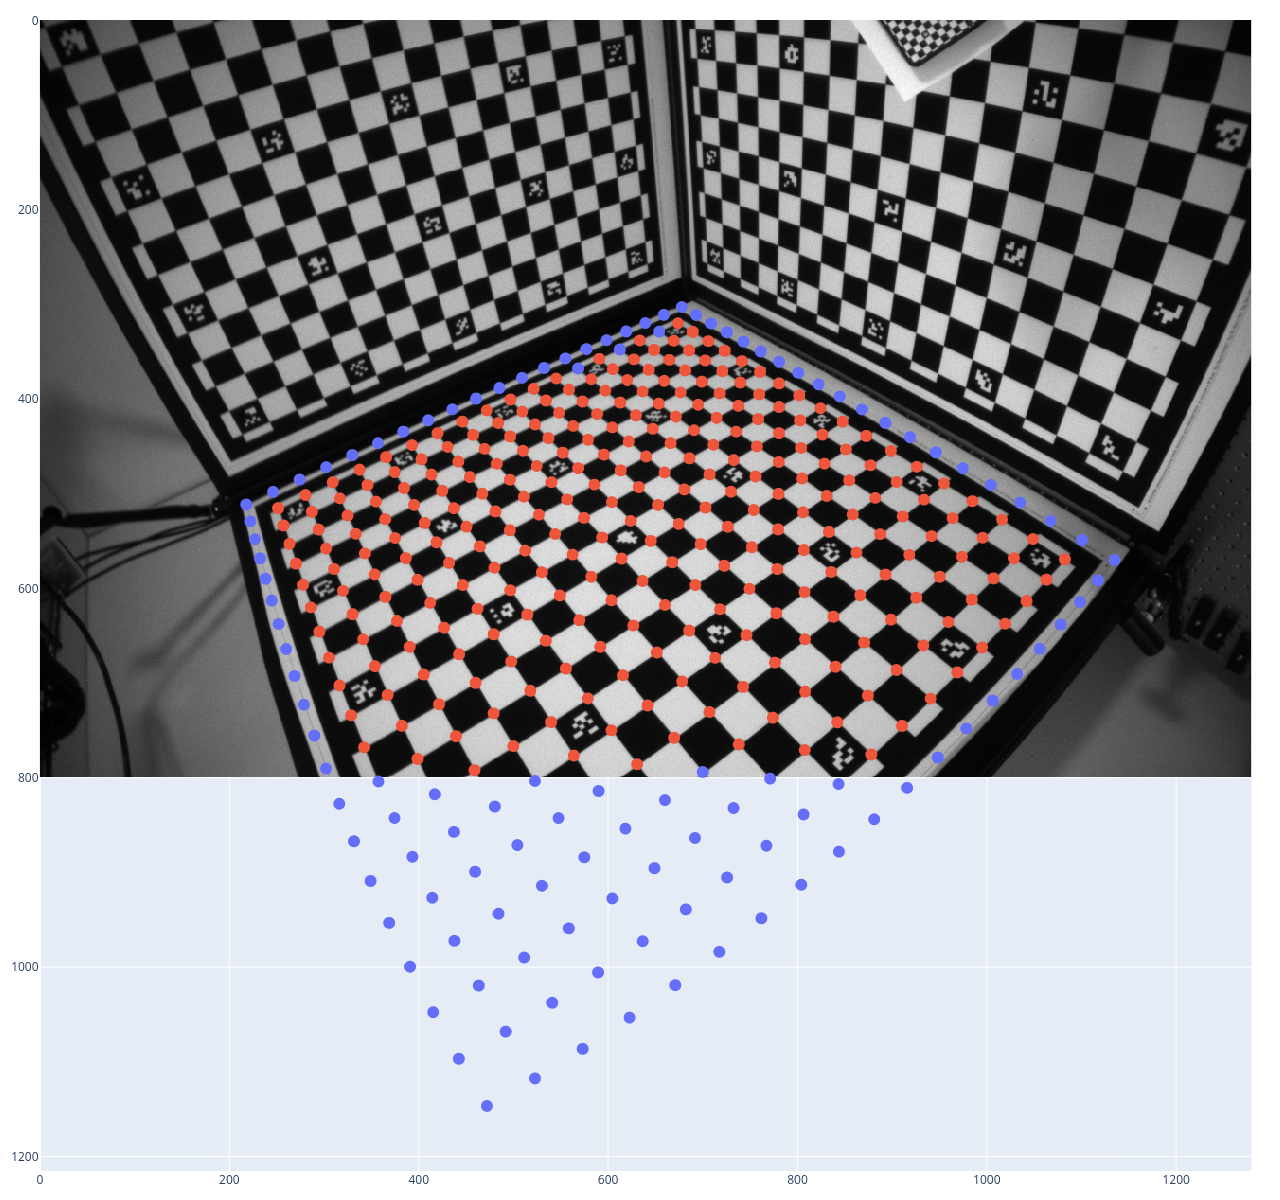
\includegraphics[width=\textwidth]{extended_board_img.png}
				\caption{Extended board, new points are marked as blue}
				\label{fig:extended_board_img}
			\end{figure}
		\end{column}
		\begin{column}{0.4\textwidth}
			\begin{figure}
				\begin{subfigure}{\textwidth}
					\resizebox{\textwidth}{!}{
						\begin{tikzpicture}
							\begin{axis}[
									xlabel={$x$},
									ylabel={$y$},
									grid=major,
									title={Original board},
								]
								\addplot[
									only marks,
								] table {data/original_board.txt};
							\end{axis}
						\end{tikzpicture}
					}
					% \caption{Original board}
				\end{subfigure}
				\begin{subfigure}{\textwidth}
					\resizebox{\textwidth}{!}{
						\begin{tikzpicture}
							\begin{axis}[
									xlabel={$x$},
									ylabel={$y$},
									grid=major,
									title={Extended board},
								]
								\addplot[
									only marks,
								] table {data/extended_board.txt};
							\end{axis}
						\end{tikzpicture}
					}
					% \caption{Extended board}
				\end{subfigure}
			\end{figure}
		\end{column}
	\end{columns}

\end{frame}

\begin{frame}
	\frametitle{Classification}

	The Hessian approach proved to be more robust, as the other gave too many false
	positives, especially for the edges.

	\begin{figure}
		\begin{subfigure}{0.30\linewidth}
			\begin{tikzpicture}[spy using outlines={circle,yellow,magnification=10,size=3cm, connect spies}]
				\node[anchor=south west,inner sep=0] (image) at (0,0)
				% {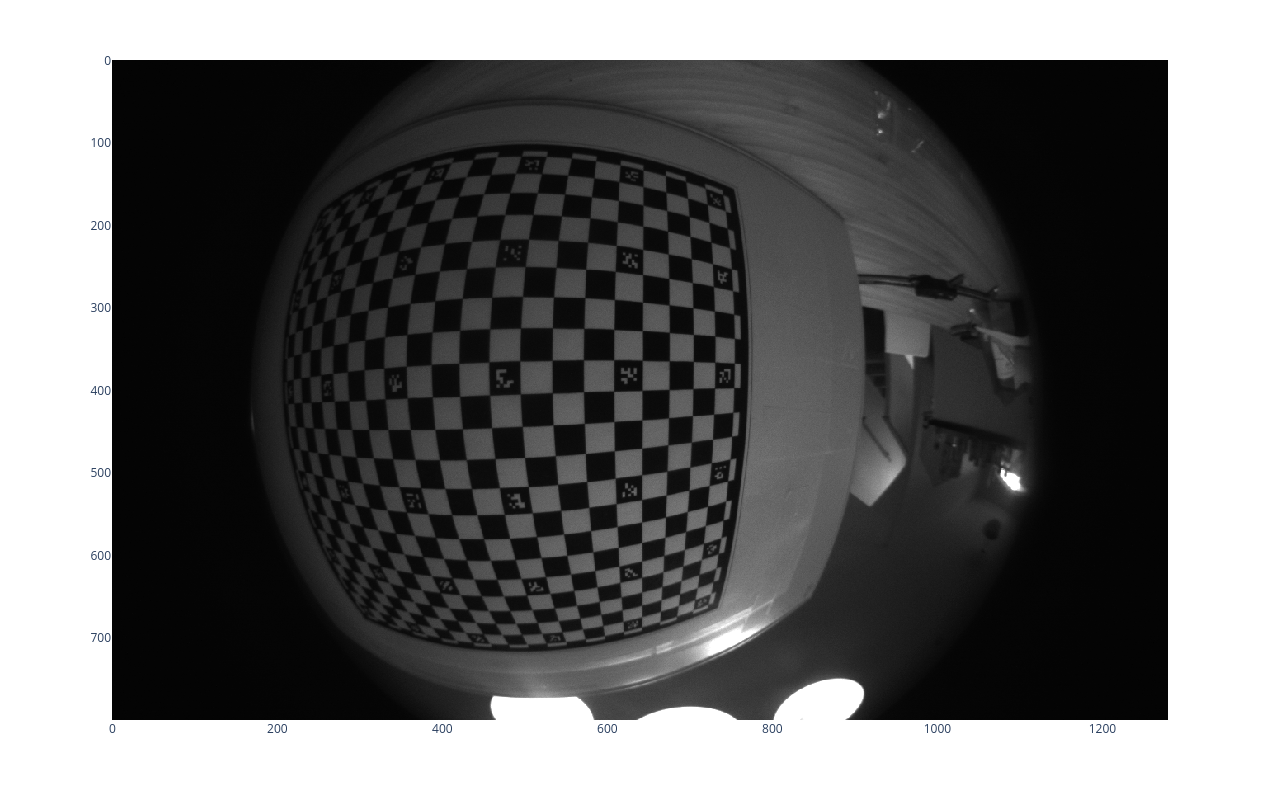
\includegraphics[width=0.10\textwidth]{distorted_image}};
				{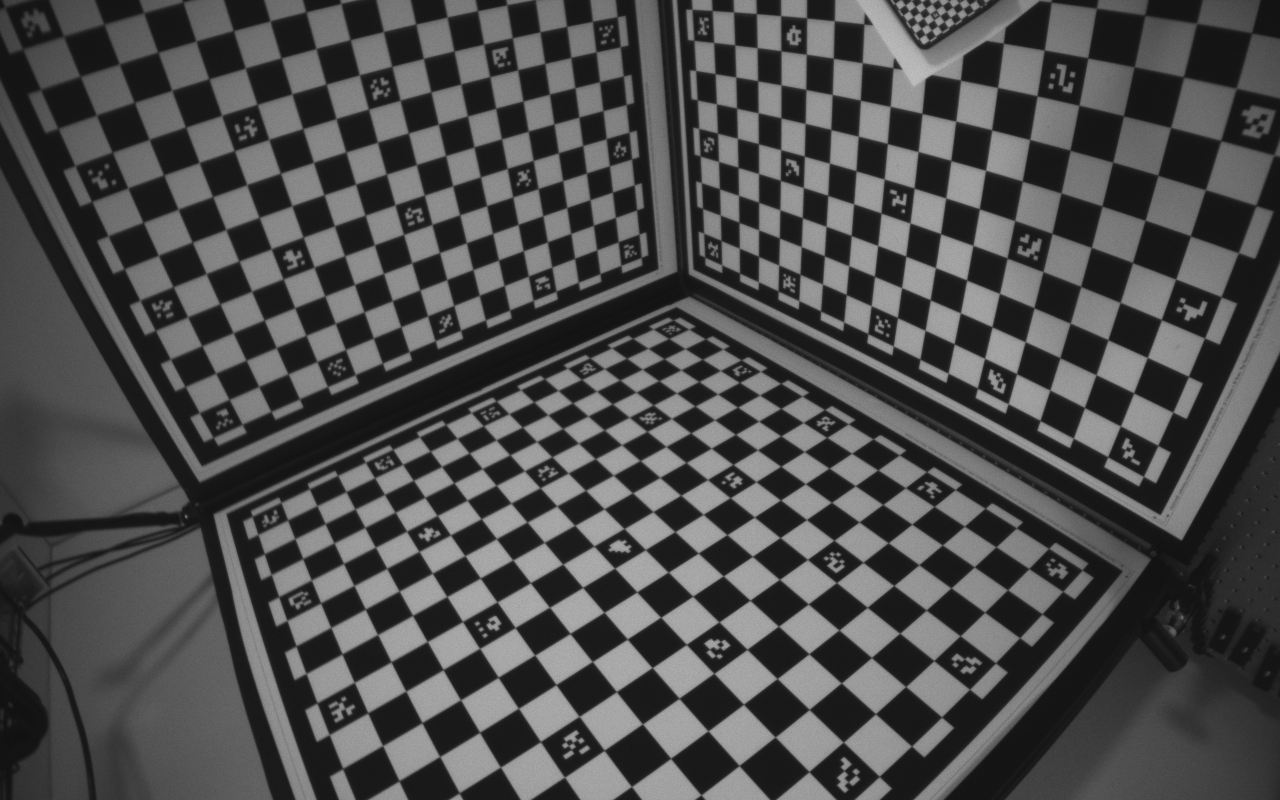
\includegraphics[width=\linewidth]{response_orig.png}};
				\begin{scope}[x={(image.south east)},y={(image.north west)}]
					\spy[red] on (1.7,1.4) in node [left] at (2.8,3.3);
					% \spy[blue] on (3.5,3.0) in node [right] at (8.1,4.3);
				\end{scope}
			\end{tikzpicture}
			\caption{Original image}
		\end{subfigure}
		\begin{subfigure}{0.30\linewidth}
			\begin{tikzpicture}[spy using outlines={circle,yellow,magnification=10,size=3cm, connect spies}]
				\node[anchor=south west,inner sep=0] (image) at (0,0)
				% {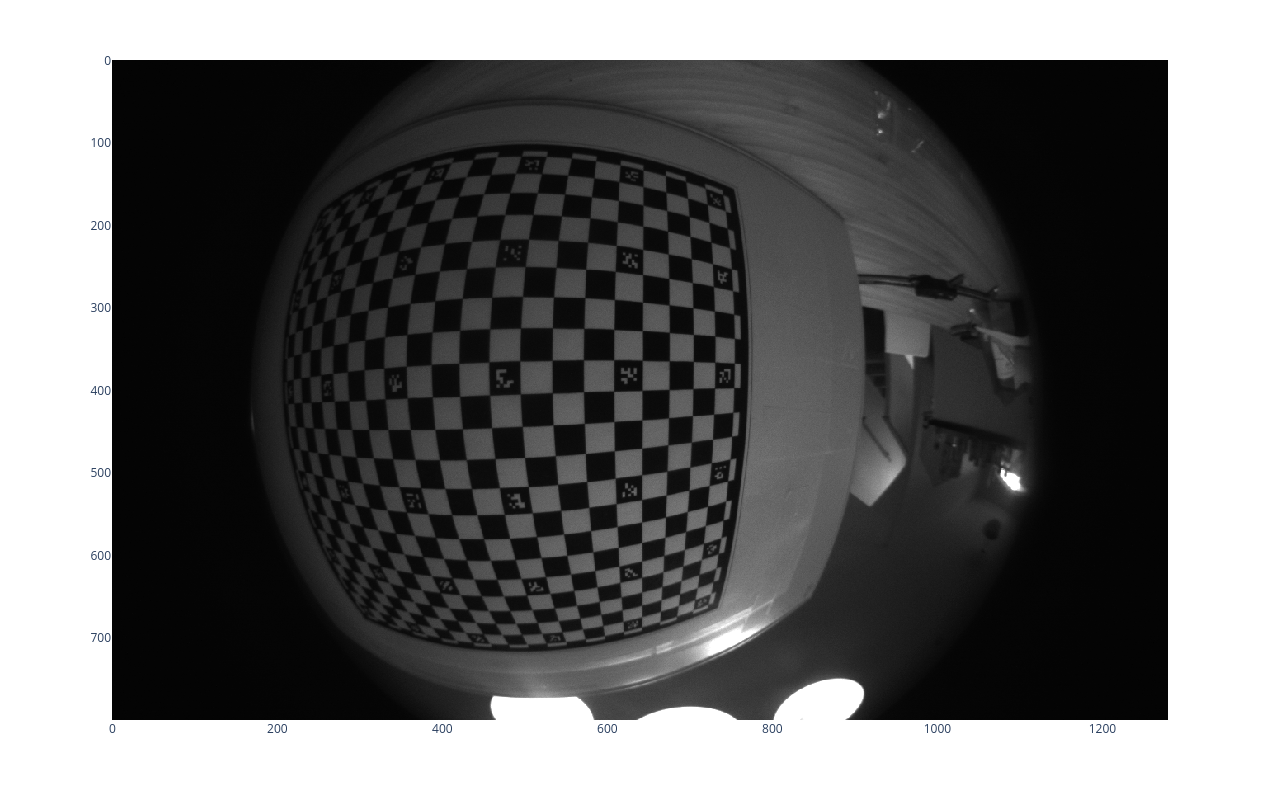
\includegraphics[width=0.10\textwidth]{distorted_image}};
				{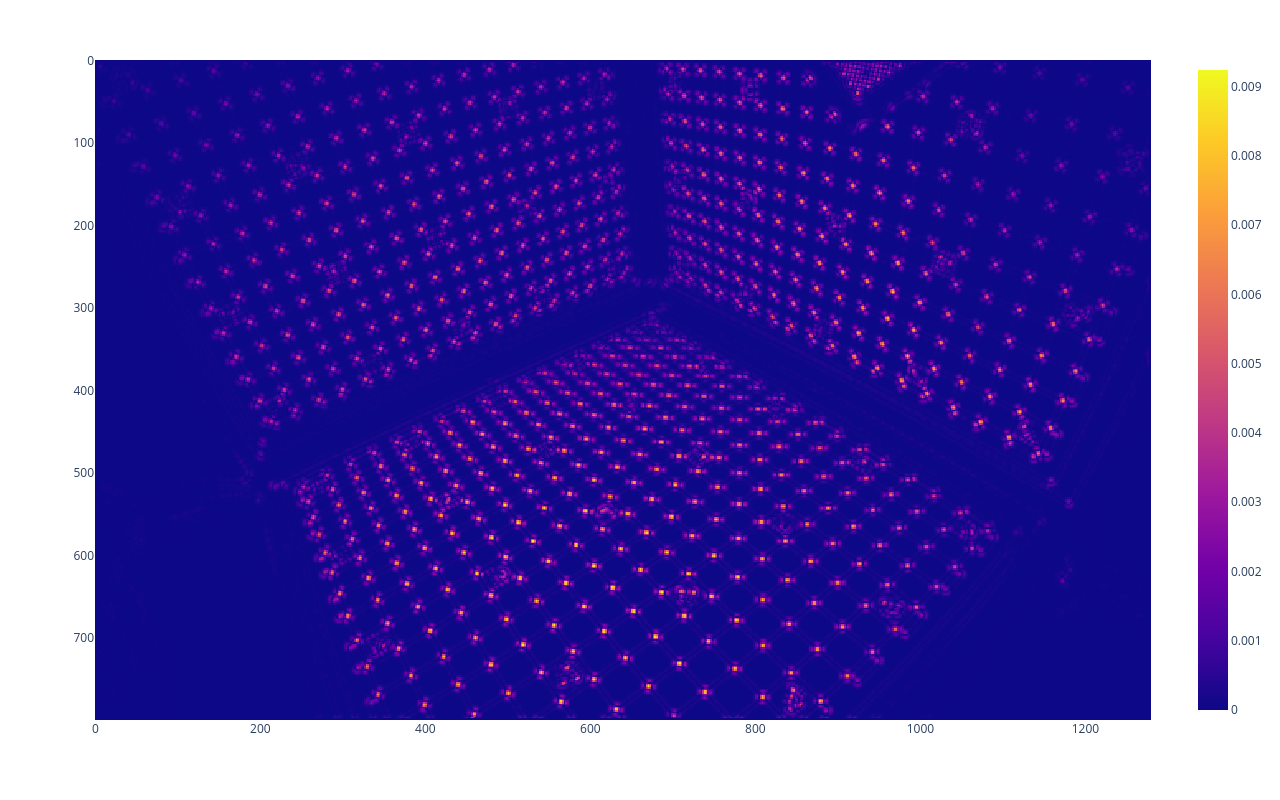
\includegraphics[width=\linewidth]{response_hessian.png}};
				\begin{scope}[x={(image.south east)},y={(image.north west)}]
					\spy[red] on (1.7,1.4) in node [left] at (2.8,3.3);
					% \spy[blue] on (3.5,3.0) in node [right] at (8.1,4.3);
				\end{scope}
			\end{tikzpicture}
			\caption{Hessian response}
		\end{subfigure}
		\begin{subfigure}{0.30\linewidth}
			\begin{tikzpicture}[spy using outlines={circle,yellow,magnification=10,size=3cm, connect spies}]
				\node[anchor=south west,inner sep=0] (image) at (0,0)
				% {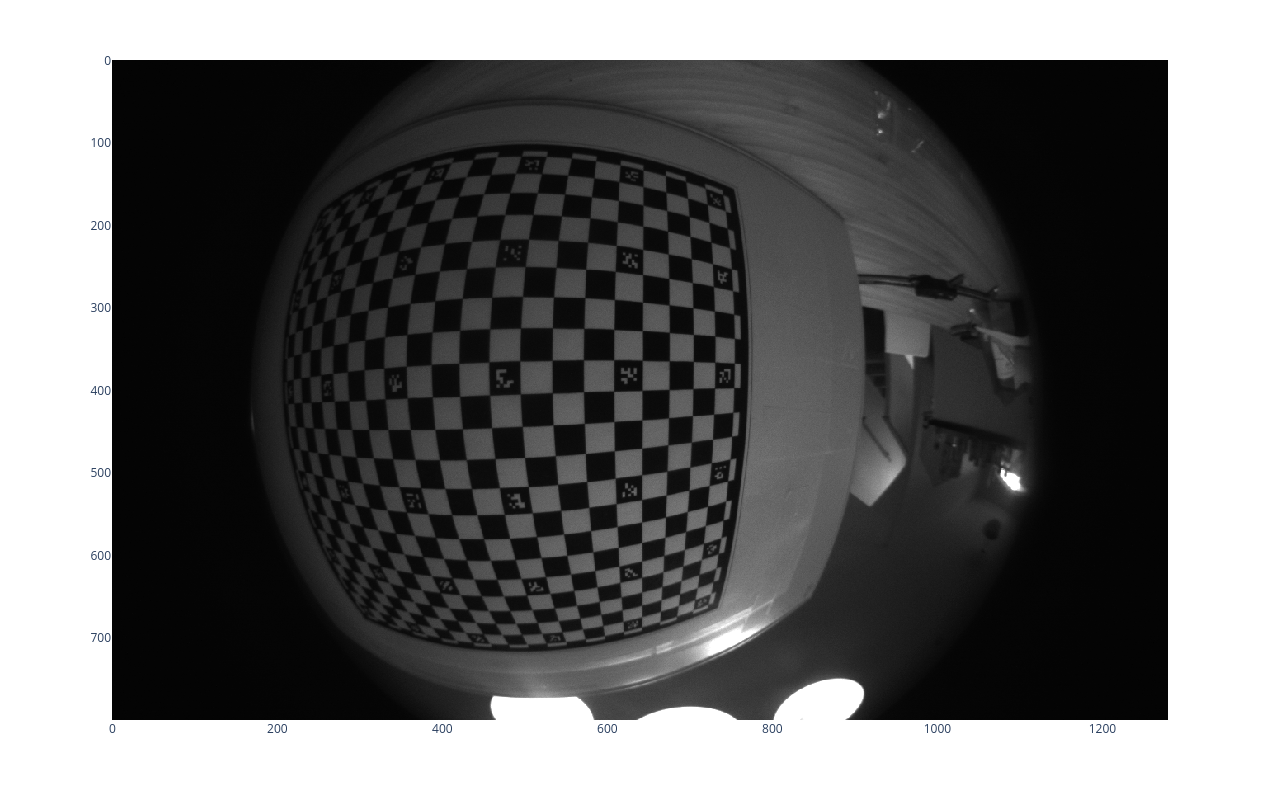
\includegraphics[width=0.6\textwidth]{distorted_image}};
				{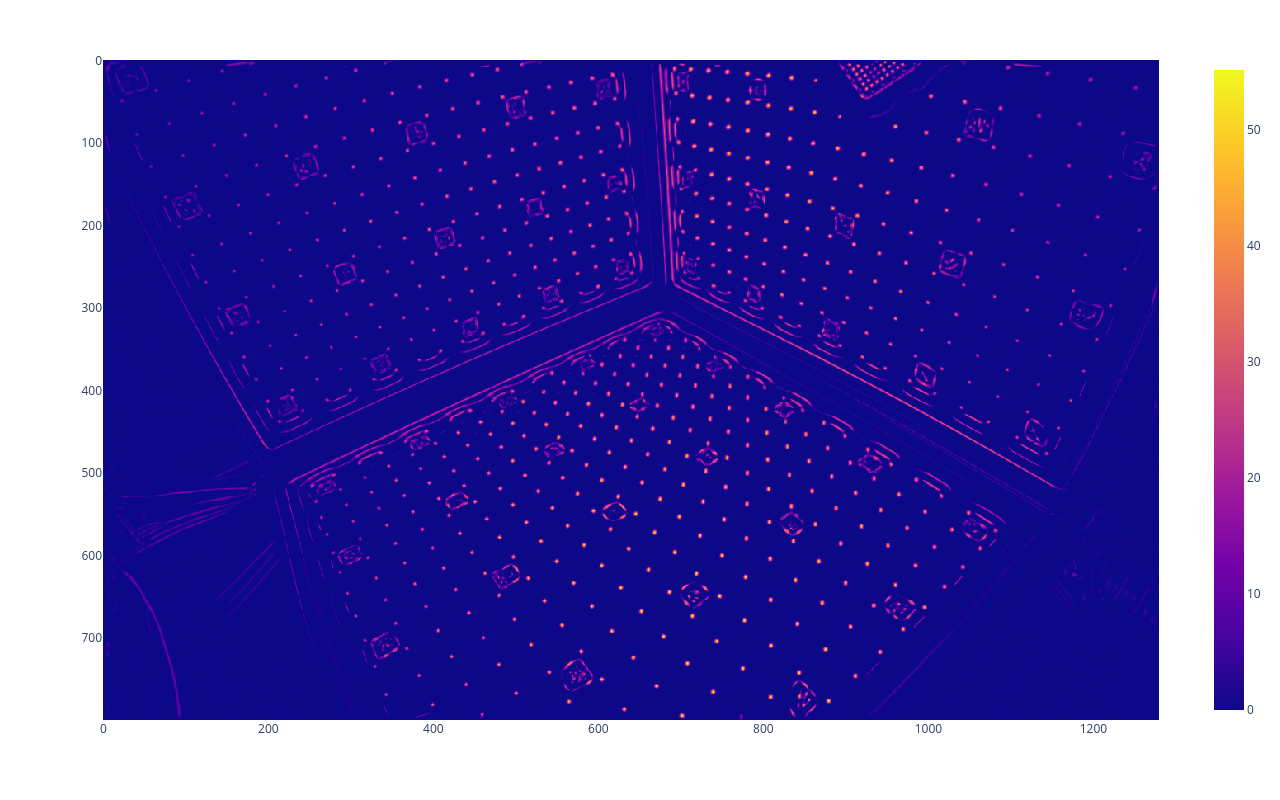
\includegraphics[width=\linewidth]{response_other.png}};
				\begin{scope}[x={(image.south east)},y={(image.north west)}]
					\spy[red] on (1.7,1.4) in node [left] at (2.8,3.3);
					% \spy[blue] on (3.5,3.0) in node [right] at (8.1,4.3);
				\end{scope}
			\end{tikzpicture}
			\caption{\cite{geigerAutomaticCameraRange2012}}
		\end{subfigure}
	\end{figure}

\end{frame}

\begin{frame}
	\frametitle{Evaluation (artificially removed points)}
	We removed 20\% of the points from the original board and then tried to recover
	them.

	\begin{figure}[h]
		\centering
		\begin{subfigure}[h]{\linewidth}
			\resizebox{\linewidth}{!}{
				\begin{tikzpicture}
					\begin{axis}[
							ybar interval,
							ymin=0,
							ylabel={Frequency},
							xlabel={Value},
							height=0.3\linewidth,
							width=\linewidth,
							ticklabel style = {font=\tiny},
							title={Histogram of points before refinement}
						]
						\addplot+ [hist={data min=0,data max=600,bins=10}] table [y index=0]
							% \addplot+ [hist={bins=30}] table [y index=0]
							{data/pruned_number_of_features.txt};
					\end{axis}
				\end{tikzpicture}
			}
		\end{subfigure}
		\hfill
		\begin{subfigure}[h]{\linewidth}
			% \centering
			\resizebox{\linewidth}{!}{
				\begin{tikzpicture}
					\begin{axis}[
							ybar interval,
							ymin=0,
							ylabel={Frequency},
							xlabel={Value},
							height=0.3\linewidth,
							width=\linewidth,
							ticklabel style = {font=\tiny},
							title={Histogram of points after refinement}
						]
						\addplot+ [hist={data min=0,data max=600,bins=10}] table [y index=0]
							% \addplot+ [hist={bins=30}] table [y index=0]
							{data/recovered_pruned_number_of_features.txt};
					\end{axis}
				\end{tikzpicture}
			}
		\end{subfigure}
	\end{figure}

\end{frame}
\begin{frame}
	\frametitle{Evaluation (artificially removed points) 2}
	\begin{figure}
		\centering
		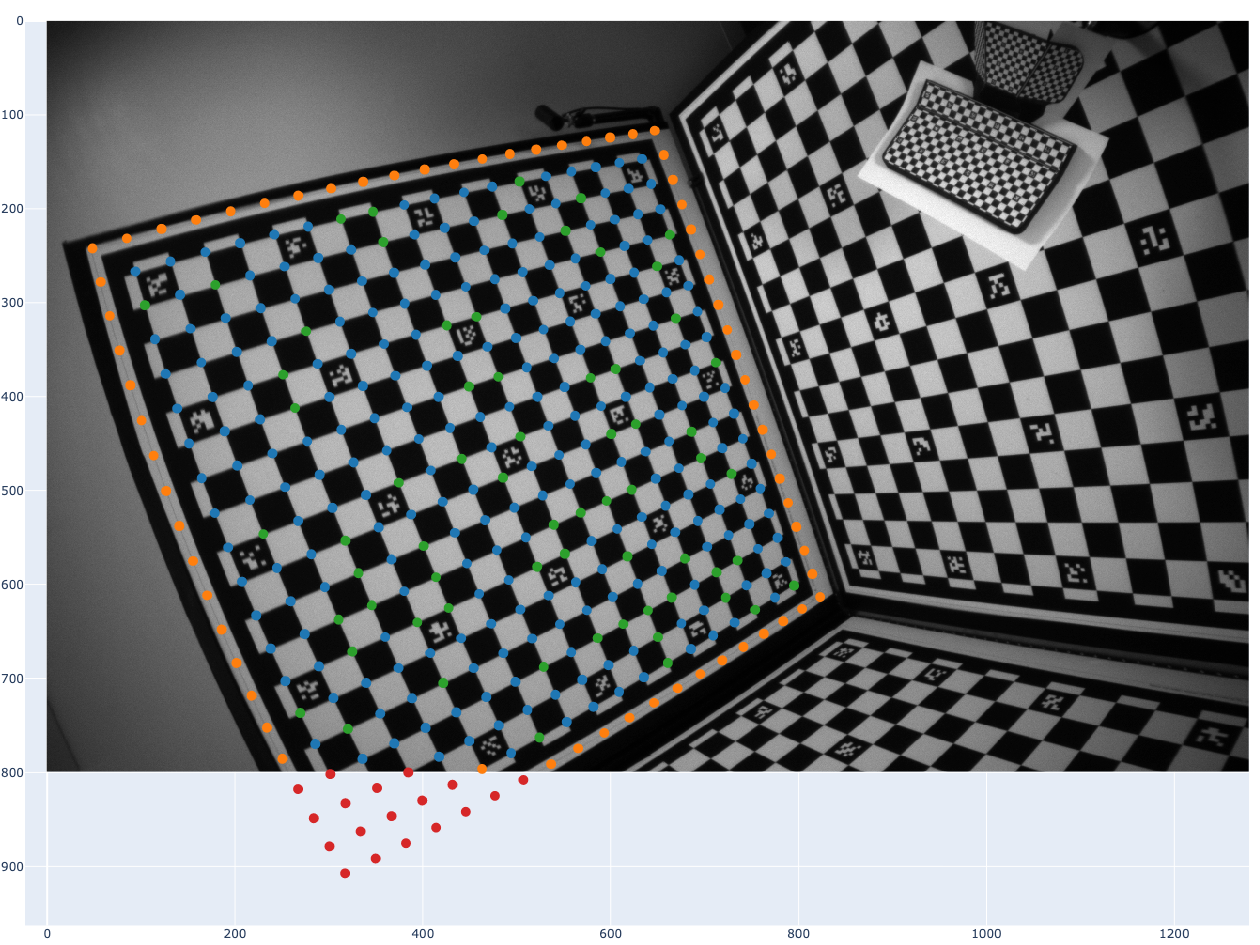
\includegraphics[width=0.7\linewidth]{refined_pruned_corners.png}
		\caption{Recovered pruned points
			(\textcolor[HTML]{1f77b4}{unchanged}
			\textcolor[HTML]{ff7f0e}{filtered out}
			\textcolor[HTML]{2ca02c}{new corner}
			\textcolor[HTML]{d62728}{out of image})}
		\caption{Feature refinement on the board with 80\% of the points}
	\end{figure}

\end{frame}

\begin{frame}
	\frametitle{Evaluation (artificial occlusion)}

	Occlusions pose additional complications for feature detection.

	\begin{figure}[h]
		\centering
		\begin{subfigure}[h]{\linewidth}
			\resizebox{\linewidth}{!}{
				\begin{tikzpicture}
					\begin{axis}[
							ybar interval,
							ymin=0,
							ylabel={Frequency},
							xlabel={Value},
							height=0.3\linewidth,
							width=\linewidth,
							ticklabel style = {font=\tiny},
							title={Histogram of points before refinement}
						]
						\addplot+ [hist={data min=0,data max=500,bins=10}] table [y index=0]
							% \addplot+ [hist={bins=30}] table [y index=0]
							{data/occluded_number_of_features.txt};
					\end{axis}
				\end{tikzpicture}
			}
		\end{subfigure}
		\begin{subfigure}[h]{\linewidth}
			% \centering
			\resizebox{\linewidth}{!}{
				\begin{tikzpicture}
					\begin{axis}[
							ybar interval,
							ymin=0,
							ylabel={Frequency},
							xlabel={Value},
							height=0.3\linewidth,
							width=\linewidth,
							ticklabel style = {font=\tiny},
							title={Histogram of points after refinement}
						]
						\addplot+ [hist={data min=0,data max=500,bins=10}] table [y index=0]
							% \addplot+ [hist={bins=30}] table [y index=0]
							{data/recovered_occluded_number_of_features.txt};
					\end{axis}
				\end{tikzpicture}
			}
		\end{subfigure}
	\end{figure}

\end{frame}
\begin{frame}
	\frametitle{Evaluation (artificial occlusion) 2}
	\begin{figure}
		\begin{subfigure}[h]{\linewidth}
			\centering
			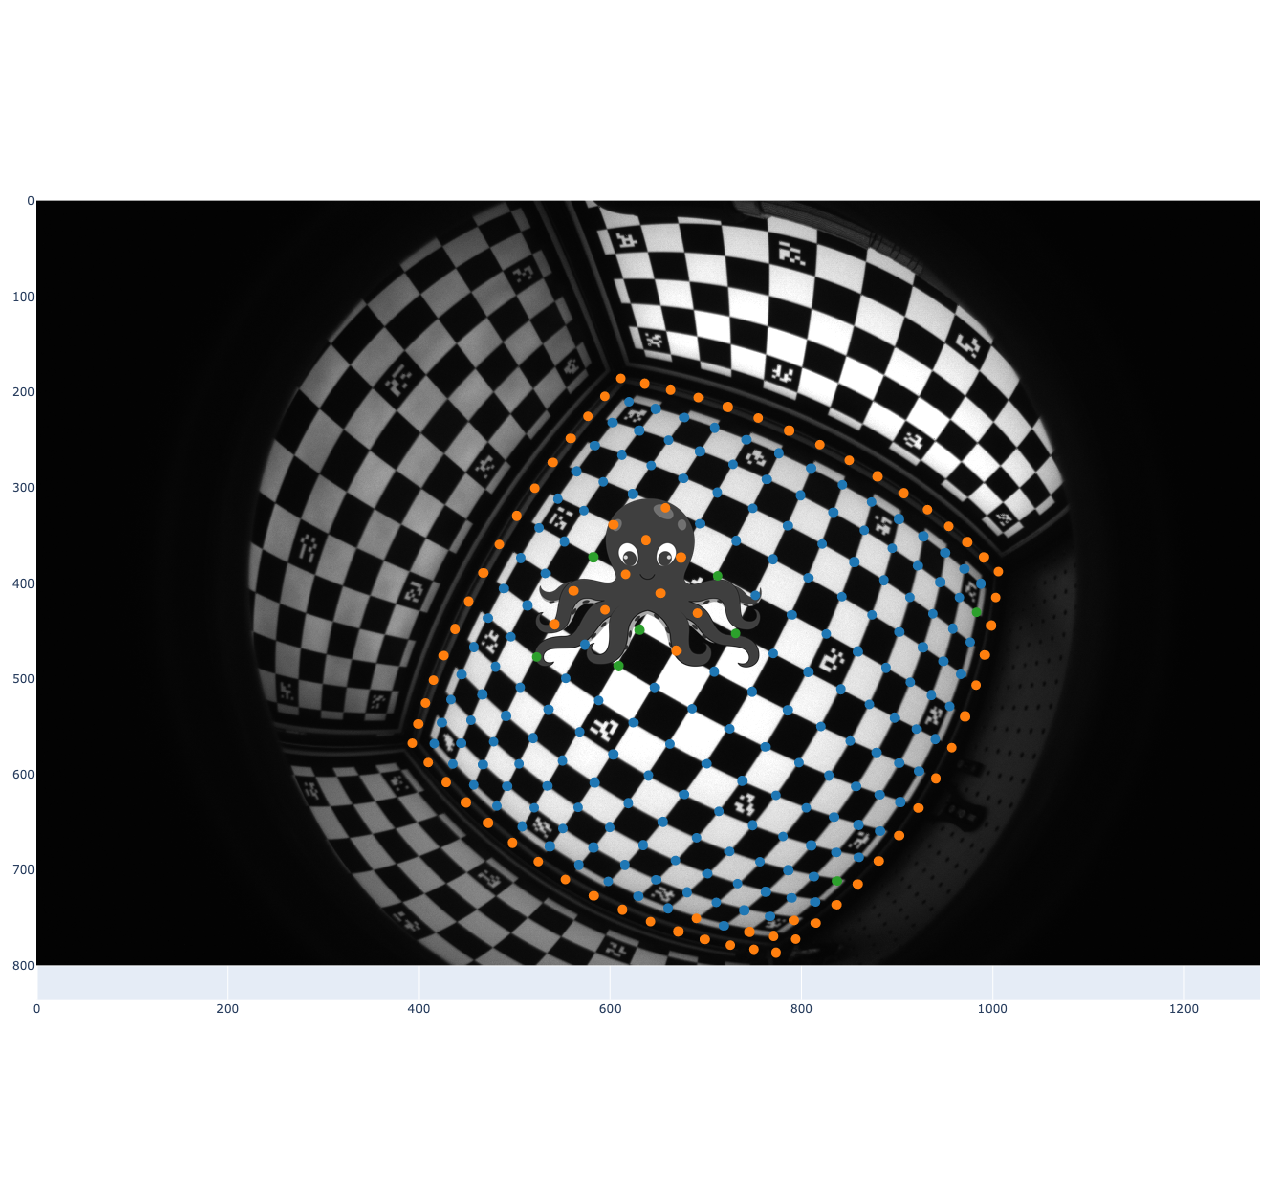
\includegraphics[width=0.7\linewidth]{refined_overlayed_corners.png}
			\caption{Recovered pruned points
				(\textcolor[HTML]{1f77b4}{unchanged}
				\textcolor[HTML]{ff7f0e}{filtered out}
				\textcolor[HTML]{2ca02c}{new corner}
				\textcolor[HTML]{d62728}{out of image})}
		\end{subfigure}
		\hfill
		\caption{Feature refinement on the board with partial board occlusion}
	\end{figure}

\end{frame}

\begin{frame}
	\frametitle{Evaluation (real data)}
	Lastly, we recovered the points that were not detected by the initial feature
	detector.

	% \begin{minipage}[t]{0.80\linewidth}
	\begin{figure}[h]
		\centering
		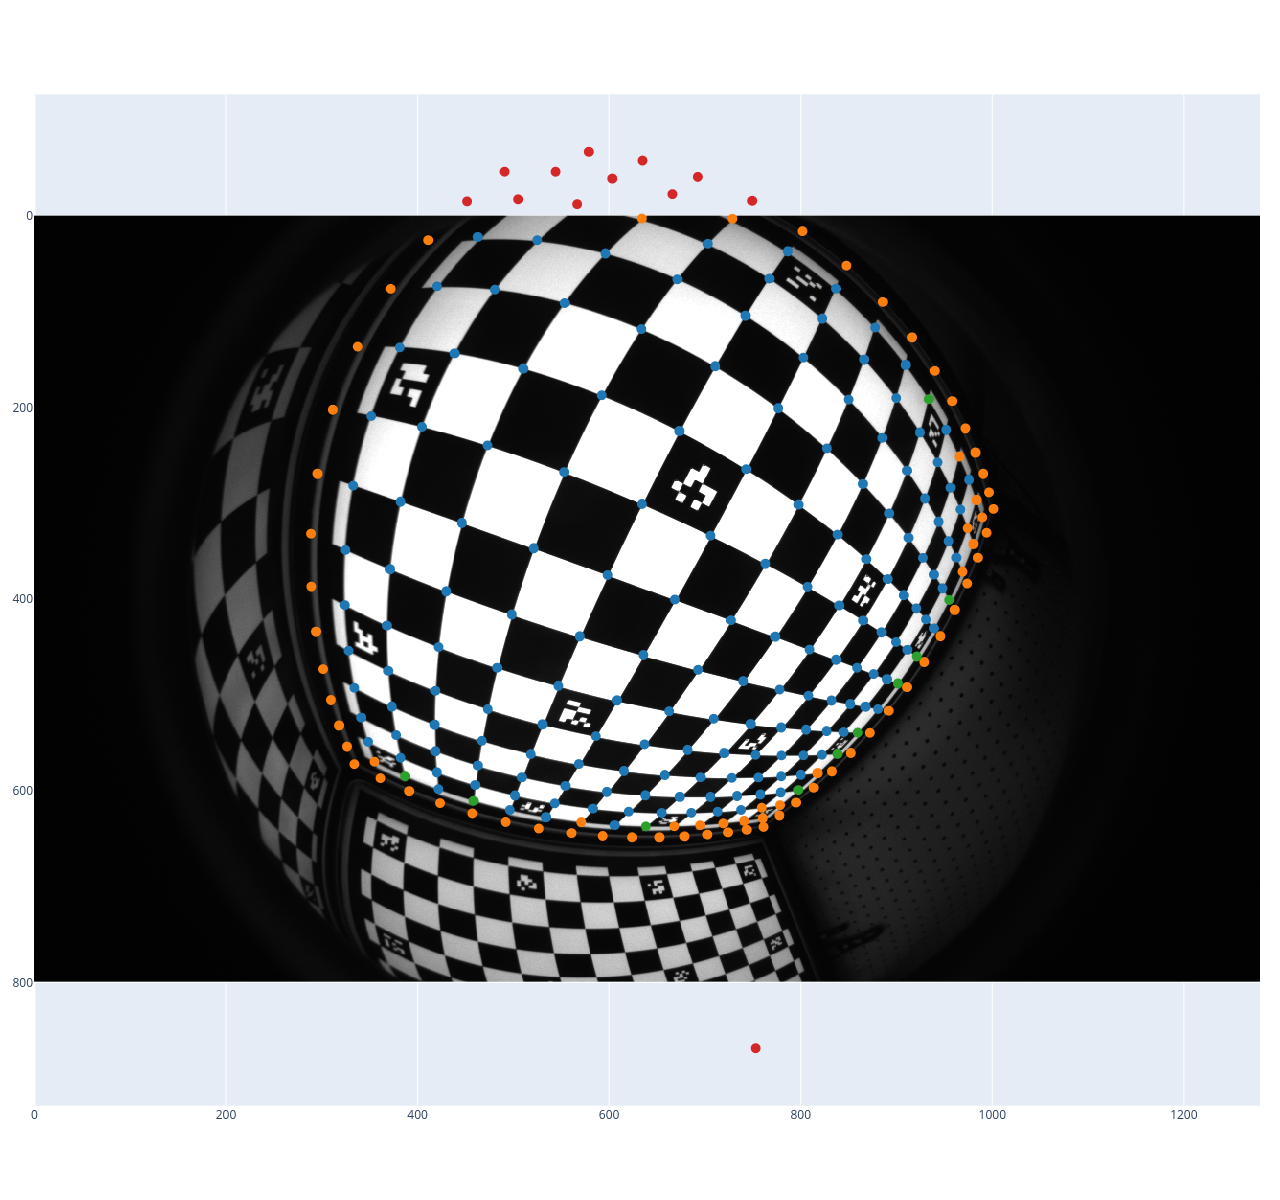
\includegraphics[width=0.75\linewidth]{refined_corners1.png}
		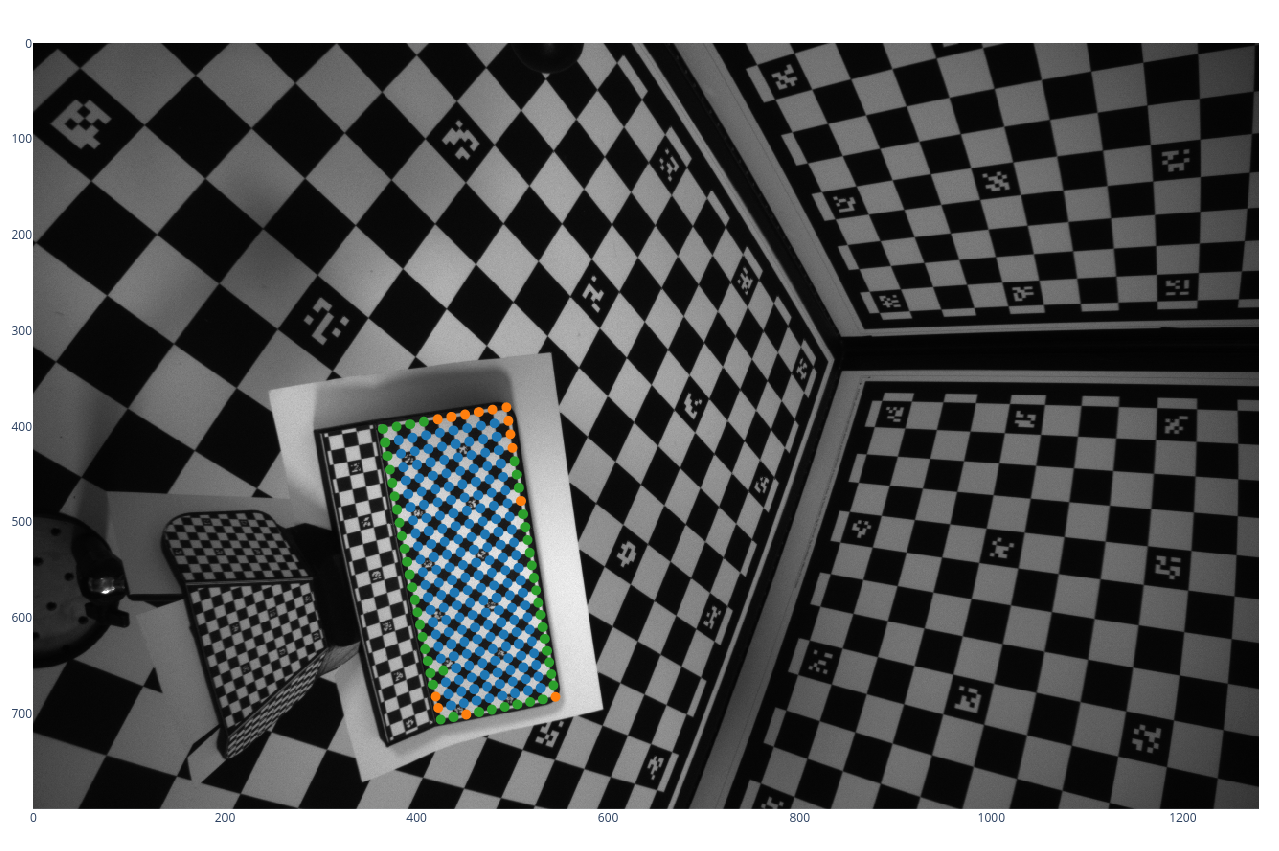
\includegraphics[width=0.75\linewidth]{refined_corners2.png}

		\caption{Recovered points
			(\textcolor[HTML]{1f77b4}{unchanged}
			\textcolor[HTML]{ff7f0e}{filtered out}
			\textcolor[HTML]{2ca02c}{new corner}
			\textcolor[HTML]{d62728}{out of image})}
		\label{fig:recovered_good_points}
	\end{figure}
	% \end{minipage}

\end{frame}

\begin{frame}
	\frametitle{Evaluation (real data, false positives) 1}

	\begin{figure}
		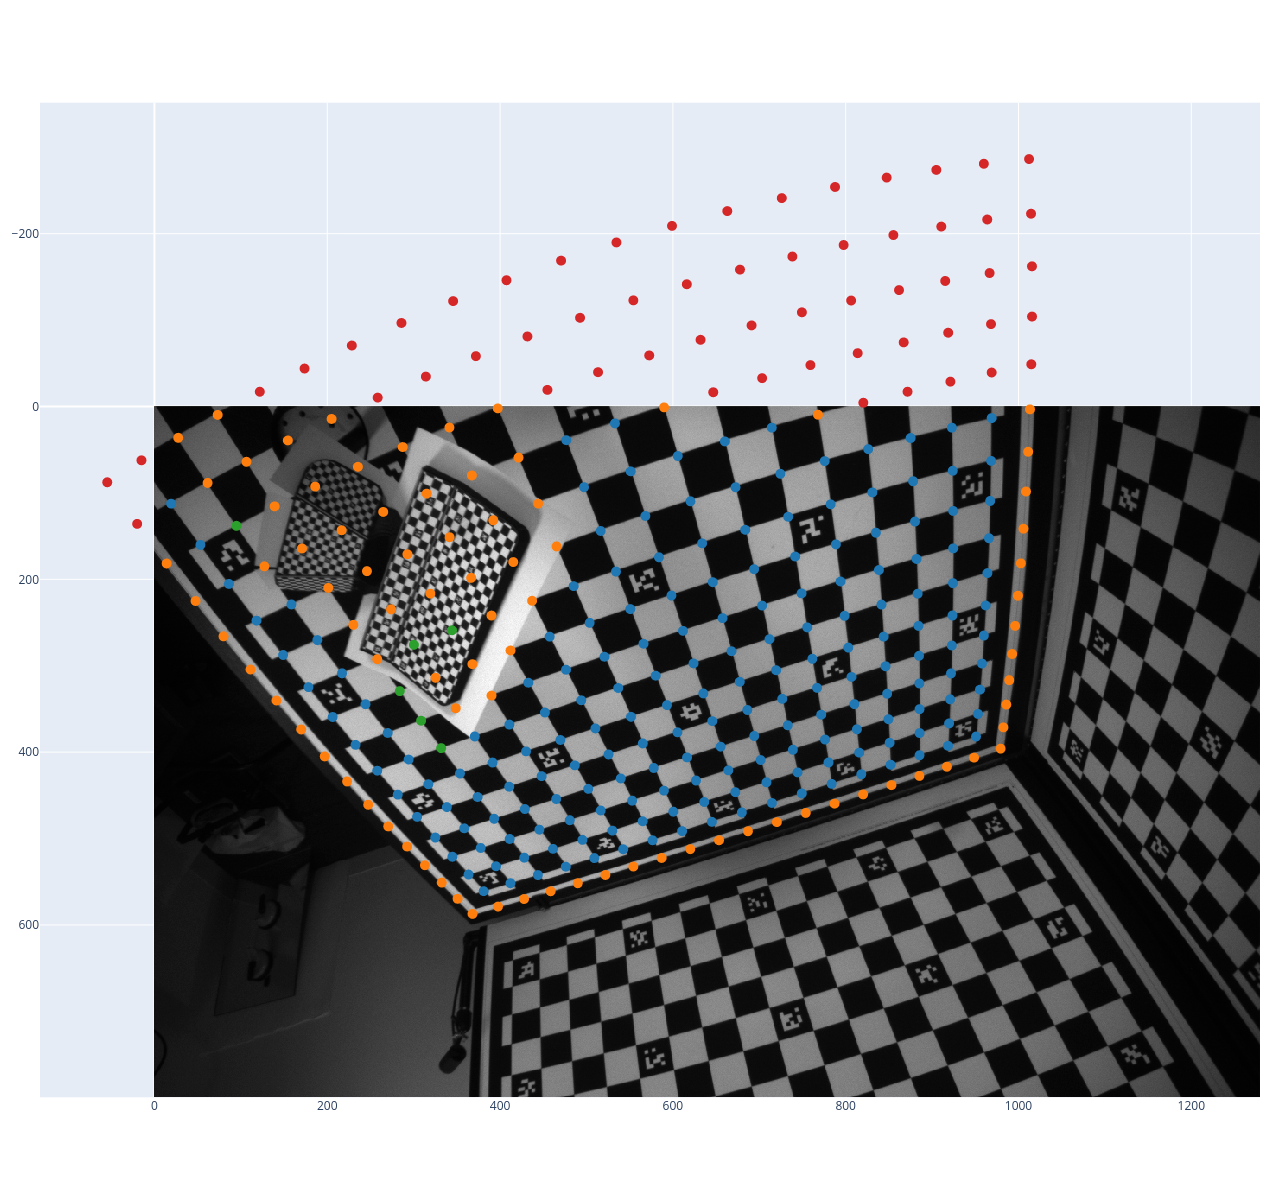
\includegraphics[width=0.8\linewidth]{refined_corners_bad.png}
		\caption{Occlusion on the board with distinct features}
	\end{figure}

\end{frame}

\begin{frame}
	\frametitle{Evaluation (real data, false positives) 2}
	\begin{figure}
		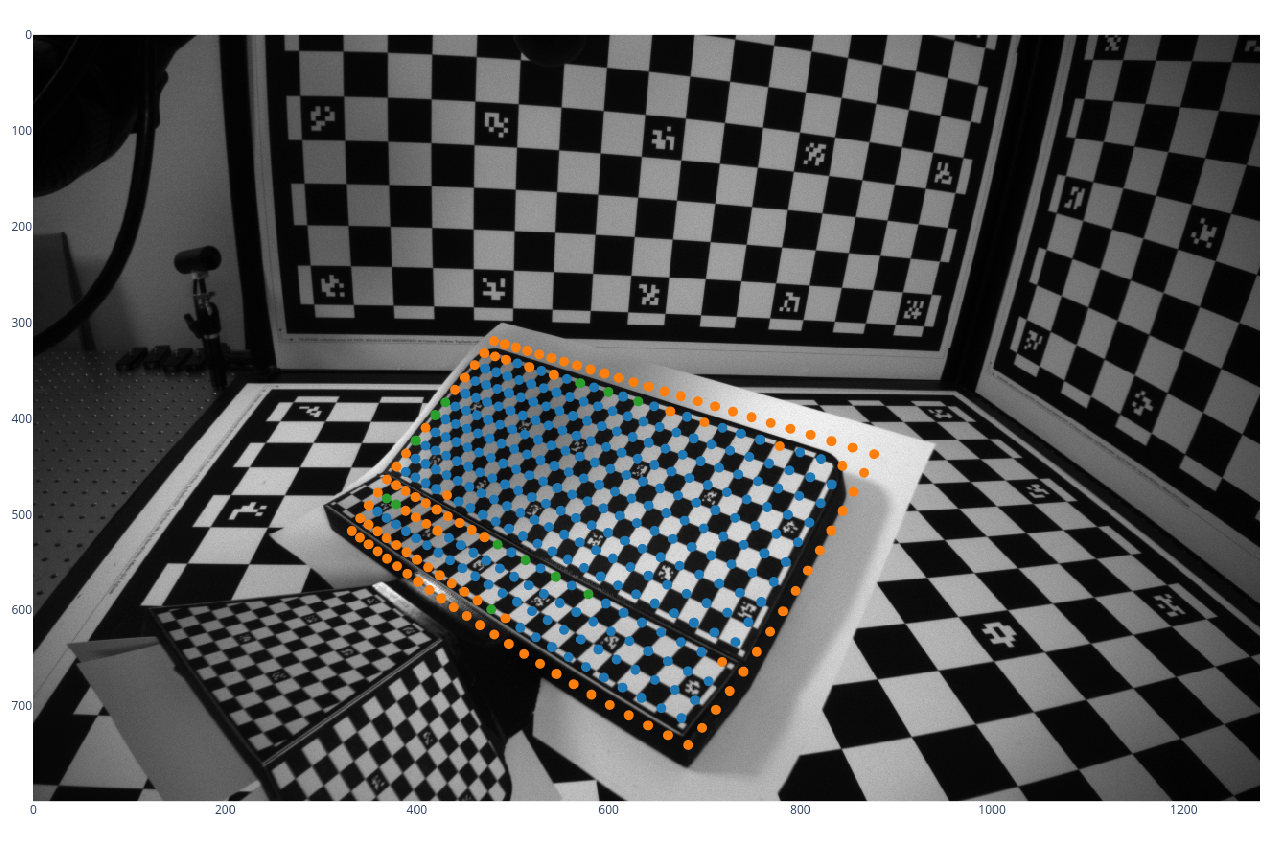
\includegraphics[width=\linewidth]{refined_corners_bad_bad.png}
		% \caption{Similar pattern to the board in the background}
	\end{figure}

\end{frame}

\begin{frame}
	\frametitle{Evaluation (real data)}

	\begin{figure}[h!]
		\begin{tikzpicture}
			\begin{axis}			[
					ymode=log,
					ybar interval,
					ylabel={Frequency},
					xlabel={Value},
					height=0.3\linewidth,
					width=\linewidth,
					ticklabel style = {font=\tiny},
					% title={Initial calibration}
				]
				\addplot+ [hist={data min=0,data max=50,bins=20}] table [y index=0]
					% \addplot+ [hist={bins=30}] table [y index=0]
					{data/number_of_refined_points.txt};
			\end{axis}
		\end{tikzpicture}
		\caption{Histogram of the newly recovered features}
		\label{fig:recovered_points_histogram}
	\end{figure}

\end{frame}

\section{Conclusions}\label{sec:conclusions}

\begin{frame}
	\frametitle{Reviewers' comments}

	\textbf{No comparison was made to classical camera calibration results and no
		discussion why results differ.}

	The main contribution is the feature detection step. The user can use the
	found camera parameters, or pass the obtained features to any camera
	calibration toolchain.
\end{frame}

\begin{frame}[standout]
	Q\&A

\end{frame}

\appendix

\begin{frame}
	\frametitle{Extrinsic parameters}
	The extrinsic parameters represent a rigid transformation from a 3-D world
	coordinate system to the 3-D camera’s coordinate system.

	\begin{exampleblock}{Definition}
		\begin{equation*}
			\widehat{\mathbf{x}} =
			R \begin{pmatrix}
				x, y, z
			\end{pmatrix}^{T} + \mathbf{t} =
			\begin{bmatrix}
				R              & \mathbf{t} \\
				\mathbf{0}^{T} & 1
			\end{bmatrix} \begin{pmatrix}
				x, y, z, 1
			\end{pmatrix}^{T},
		\end{equation*}
		where
		\(\begin{pmatrix}
			x, y, z
		\end{pmatrix}^{T}\) is a 3D scene point,
		% \(R \begin{pmatrix}
		% 	x, y, z
		% \end{pmatrix}^{T} + \mathbf{t}\), where
		\(R\) is a \(3 \times 3\) rotation matrix
		and \(\mathbf{t}\) is
		a \(3 \times 1\) translation vector.
	\end{exampleblock}
\end{frame}

\begin{frame}
	\frametitle{Extrinsic parameters}

	When working with the coplanar scene points, we can simplify the projection
	by assuming that the scene plane is located at \(Z = 0\). In this case, the
	projection of the point becomes:
	\begin{exampleblock}{Definition for coplanar points}
		\begin{equation*}
			\alpha \begin{pmatrix}
				u \\ v \\ 1
			\end{pmatrix} = \begin{bmatrix}
				\mathbf{r_1} & \mathbf{r_2} & \mathbf{r_3} & \mathbf{t}
			\end{bmatrix} \begin{pmatrix}
				x \\ y \\ 0 \\ 1
				% \end{pmatrix} = \begin{bmatrix}
				%   \mathbf{p_1} & \mathbf{p_2} & \mathbf{p_4}
				% \end{bmatrix} \begin{pmatrix}
				%   x \\ y \\ 1
				% \end{pmatrix}.
			\end{pmatrix} = \underbrace{\begin{bmatrix}
					\mathbf{r_1} & \mathbf{r_2} & \mathbf{t}
				\end{bmatrix}}_{H} \begin{pmatrix}
				x \\ y \\ 1
			\end{pmatrix}.
		\end{equation*}
	\end{exampleblock}
\end{frame}

\begin{frame}
	\frametitle{Distortion model}
	The distortion of the image is caused by the lens not being perfectly planar.
	We used the division distortion model
	\cite{fitzgibbonSimultaneousLinearEstimation2001} which maps a
	point from a retinal plane to the
	ray direction in the camera coordinate system.
	\begin{exampleblock}{Definition}
		\begin{equation*}
			g(\mathbf{u}) = \begin{pmatrix}
				u, v, \psi(r(\mathbf{u}))
			\end{pmatrix}^{T},
			\psi(r) = 1 + \sum_{n = 1}^{N} \lambda_n r^{2n},
		\end{equation*}
		where
		\(\mathbf{u} = \begin{pmatrix}
			u, v, 1
		\end{pmatrix}^{T}\) is a point in the retinal plane
		, \(r(\mathbf{u}) = \sqrt{u^2 + v^2}\) is the radial distance from the
		principal point and \(\lambda_n\) are the distortion coefficients.
	\end{exampleblock}
\end{frame}

\begin{frame}
	\frametitle{Intrinsic parameters}
	Represent a projective transformation from the 3-D camera’s coordinates into
	the 2-D image coordinates.

	\begin{exampleblock}{Definition}
		\begin{equation*}
			K = \begin{bmatrix}
				\alpha_x & \alpha_x \cot \theta & c_x \\
				0        & \alpha_y             & c_y \\
				0        & 0                    & 1
			\end{bmatrix} \begin{bmatrix}
				f & 0 & 0 \\
				0 & f & 0 \\
				0 & 0 & 1
			\end{bmatrix} = \begin{bmatrix}
				f_x & k   & c_x \\
				0   & f_y & c_y \\
				0   & 0   & 1
			\end{bmatrix}.
		\end{equation*}
		For a typical camera, \(\theta = \sfrac{\pi}{2}\) and \(\alpha_x = \alpha_y\)
		\cite{hartleyMultipleViewGeometry2004}:
		\begin{equation*}
			K = \begin{bmatrix}
				f & 0 & c_x \\
				0 & f & c_y \\
				0 & 0 & 1
			\end{bmatrix}.
		\end{equation*}
	\end{exampleblock}

\end{frame}

\end{document}
